% !TeX encoding = UTF-8
% !TeX root = ../Vitamintablettenspender.tex

\chapter{Konzeptionierung}

Im Entwicklungsprozess nimmt die Suche nach der optimalen Lösung für das vom Kunden gewünschte Produkt die Hauptaufgabe ein. Das Ergebnis soll nachvollziehbar und objektiv bewertbar sein. Dafür wird im Folgenden zunächst eine umfassende Planung des Produktes hinsichtlich Markt- und Wettbewerbschancen durchgeführt.

Die Entwicklung des Konzepts erfolgt darauffolgend anhand eines Projektplans, der den vom Kunden gewünschten Termin zur Vorstellung des Produktes mit einem Prototypen berücksichtigt. In der Anforderungsliste werden die Anforderungen des Kunden aus dem Lastenheft konkretisiert und durch interne Spezifikationen ergänzt. Damit wird eine Basis zur Entwicklung von Lösungsideen geschaffen.

Hierfür werden zunächst die Zusammenhänge von Anforderungen und Funktionen abstrakt in der Funktionsstruktur dargestellt, wobei das Loslösen vom Gegenständlichen und von vorzeitigen Festlegungen auf ein bestimmtes Lösungskonzept ermöglicht wird. Zur Systematisierung der Suche und Auswahl des optimalen Lösungsprinzips wird im morphologischen Kasten alle Lösungsoptionen aller Teilfunktionen berücksichtigt und verschiedene Gesamtlösungskombinationen unter Beachtung von Konflikten untereinander gebildet. Die abgesicherte Festlegung des zu realisierenden Lösungskonzeptes erfolgt in der Nutzwertanalyse. Zuletzt wird ein Grobentwurf zur Verdeutlichung des Wirkprinzips angefertigt.

\section{Produktplanung}
Der Markt für Nahrungsergänzungsmittel ist riesig. Mehrere Studien und Umfragen zeigten bereits die enorme Nachfrage deutschlandweit. So wurden nach einer Studie von Insight Health \cite{studie1}, die auf der Website des deutschen Lebensmittelverbandes veröffentlicht wurde, dass im Jahr 2018 225 Millionen Packungen Nahrungsergänzungsmittel verkauft wurden. Das entspricht einem Umsatz von circa 1,439 Milliarden Euro. Dabei machen Vitamine und Mineralstoffe näherungsweise zwei Drittel des gesamten Nahrungsergänzungsmittel-Marktes aus. Das Vitamin C, zur Stärkung des Immunsystems, ist dabei in der Sparte der Vitaminprodukte mit großem Abstand am beliebtesten, sodass davon im Jahr 2019 29,2 Millionen Packungen abgesetzt wurden. Zweitplatziert sind Multivitamin-Tabletten mit Mineralstoffen, die immer noch 17,5 Millionen verkaufte Packungen vorweisen können. Aber auch Vitamintabletten, die lediglich das Vitamin B12 oder die Vitamine A/D oder B-Komplexe beinhalten, sind sehr stark gefragt.

Unabhängig von Vitaminen werden einige Mineralstoffe wie Magnesium insbesondere für Sportler oder Calcium vom Markt aufgekauft. Dabei wurden im Jahr 2018 36,8 Millionen Packungen Magnesium sowie 16,4 Millionen Packungen Calcium verkauft. Die Chancen, dass ein Produkt zur automatisierten Ausgabe von Tabletten mit Vitaminen und Mineralen vertrieben wird, sind damit gegeben. Die bereits große Akzeptanz von Medikamentendispensern stellen ein gutes Beispiel für die Erfolgsaussichten des zu entwickelnden Produktes. Diese Dispenser verringern die Wahrscheinlichkeit falsche Medikamente einzunehmen und bieten dabei zeitgleich einen hohen Komfort. Mit dem Vitamintablettenspender wird ein Produkt konstruiert, das der breiten Masse der Bevölkerung zugänglich gemacht werden kann. Aufgrund der hohen Verkaufszahlen von Nahrungsergänzungsmitteln bieten sich Chancen durch den erhöhten Komfort der Tablettenzubereitung und der damit erleichterten Einnahme. Außerdem kann die Aufbewahrung verschiedener Vitamin- und Mineralsorten die Vielfältigkeit in der Nachfrage nach Nahrungsergänzungsmitteln kompensieren.

Die Technologien zum Realisieren des Produktwunsches sind gegeben. Es gibt zahlreiche Möglichkeiten zum Entwerfen eines Ausgabemechanismus von Vitamintabletten. Da technologisch größtenteils nur Motoren zum Erzeugen des gewünschten Schiebeprinzips eingesetzt werden müssen, treten bei der Umsetzung ausschließlich Komponenten der Technologien aus dem Bereich der Basis- oder der Alten Technologien auf. Diese sind preislich günstig zu bekommen und können durch geschickte Kombination miteinander Gewinne einbringen. Beispielsweise wurden in Norwegen im Jahr 2018 elektronische Medikamentendispenser in Krankenhäuser in einem Pilotprojekt getestet \cite{studie2}, wodurch bestätigt wird, dass die technischen Voraussetzungen für das Produkt gegeben sind.

Im direkten Wettbewerb mit dem automatischen Vitamintablettenspender steht ein Produkt der Firma Tespo (Plymouth, England), das die automatische Ausgabe ihrer eigenen Vitaminprodukten in Pulverform ermöglicht. Dieses Produkt ist jedoch nicht für den Massenmarkt und herkömmliche Vitamintabletten geeignet. Des Weiteren gibt es Behältnisse zu Aufbewahrung von Tabletten. Diese stellen jedoch nicht die automatische Ausgabe sowie das anschließende Auffüllen des Trinkbehältnisses mit Wasser bereit. Die gewünschte Bedienbarkeit mit einem Touchdisplay sind zusammen mit der automatischen Zubereitung Alleinstellungsmerkmale. Damit ist das Produkt ein Unikat und hebt sich gegenüber der Konkurrenz deutlich ab.

In der Patentanalyse wurde mittels der Bottom-Up-Recherche-Methode sichergestellt, dass es keine vergleichbaren Patente des Produkts gibt. Dabei wurden im Depatisnet, Espacenet sowie unter Google Patents keine relevanten Produkte gefunden. Es existiert ausschließlich das deutsche Patent DE000029811862U1 mit dem Titel "Vitamin-Tablettenspender". Das im Jahr 1998 angemeldete Gebrauchsmuster beschreibt einen Spender, an dem Tablettenröhrchen befestigt werden können. Mit Hilfe eines mechanischen Schiebers können einzelne Tabletten herausgenommen werden. Für die Konstruktion ist die Montage an der Wand vorgesehen, wobei dort die einzelnen Tablettenröhrchen ausgetauscht werden können. Das Patent beinhaltet das Funktionsprinzip des zu entwickelnden Produktes nur eingeschränkt. Geschützt wird eine komplette Wandhalterung, bei der die Befestigung mittels Verschrauben der Produktschenkel erfolgt.

Des Weiteren wird die direkte Montage der Röhrchen sowie der mechanischen Schieber zum Herausnehmen der Tabletten patentiert. Das zu entwickelnde Produkt erweitert das Prinzip in seiner Funktion, sodass der Wirkbereich des Schutzes verlassen wird. Der automatische Prozess zur Tablettenausgabe löst dabei den Schiebemechanismus ab, sollte jedoch hinsichtlich seiner Ähnlichkeit zum mechanischen Schieber überprüft und abgesichert werden. Das System ist nicht zur Montage an der Wand vorgesehen. Außerdem ist die Befüllung des Gerätes mit den Tabletten angedacht, sodass die einzelnen Röhrchen nicht direkt am Produkt montiert werden. Durch Hinzufügen von wesentlichen Produktfunktionen wie beispielsweise einem Touchscreen, einem Wasserbehälter zum automatischen Auffüllen des Trinkbehälters und einigen weiteren Zusatzfunktionen hebt sich das System deutlich vom Patent ab und kann konstruiert werden. Die Kombination der einzelnen Komponenten für sein Anwendungsgebiet kann als Patent angemeldet werden.

\section{Projektplan}
\begin{figure}[H]
	\centering
	\includegraphics[angle=90, height=0.9\textheight]{chapter/Bilder/ganttplan} 
	\caption{Projektplan}
\end{figure}

\section{Anforderungsdefinition}

\newcolumntype{L}[1]{>{\raggedright\arraybackslash}p{#1}} % linksbündig mit Breitenangabe
\newcolumntype{C}[1]{>{\centering\arraybackslash}p{#1}} % zentriert mit Breitenangabe
\newcolumntype{R}[1]{>{\raggedleft\arraybackslash}p{#1}} % rechtsbündig mit Breitenangabe

\begin{longtable}{C{0.03\linewidth}C{0.05\linewidth}C{0.05\linewidth}L{0.5\linewidth}C{0.14\linewidth}C{0.07\linewidth}}
	\toprule
 	
 	\textbf{Nr.} & \textbf{F/W} & \textbf{Gew.} & \textbf{Beschreibung und Erläuterung} & \textbf{Faktortyp} & \textbf{Ver.}\\
	
	\toprule
	\endfirsthead
	
	\textbf{1} & & & \textbf{Funktionsanforderungen} && \\
	1.1 & F & & Automatische Ausgabe einer Vitamintablette nach Wahleingabe über einen Auswurf in einen Trinkbehälter & Basis & KK/TG\\
	1.2 & W & 9 & Ausgabe sollte innerhalb 15 Sekunden nach Wahleingabe erfolgen & Leistung & KK/TG\\
	1.3 & W & 6 & Automatische Ausgabe einer Tablette bei Platzierung eines Trinkbehälters unter den Auswurf&Begeisterung& KK/TG\\
	1.4 & W & 10 & Automatisches Auffüllen des Trinkbehälters mit Wasser nach Tablettenausgabe &Begeisterung& KK/TG\\
	1.5 & W & 4 & Es sollte nur eine der Tageszeit entsprechende Tablette ausgegeben werden, um die Vitaminbalance des Nutzers zu garantieren &Begeisterung& KK/TG \\
	1.6 & F & & Aufbewahrungs- und Ausgabemöglichkeit für mindestens zwei unterschiedliche Vitamintablettensorten & Basis & KK/TG\\
	1.7 & F & & Aufbewahrungsmöglichkeit für mindestens 20 Brausetabletten je Vitamintablettensorte & Basis & KK/TG\\
	1.8 & F & & Anzeige der aktuellen Uhrzeit & Basis & KK/TG\\
	1.9 & W & 5 & Anzeige des nächsten Tablettentyps, der vom Nutzer eingenommen werden soll, um eine regelmäßigen Tabletteneinnahme zu überwachen &Begeisterung& KK/TG\\
	1.10 & W & 4 & Anzeige der Uhrzeit für die vom Nutzer als nächstes zu nehmende Tablette &Begeisterung& KK/TG\\
	1.11 & W & 3 & Warnton, wenn Uhrzeit von Anforderung 1.10 für einen Nutzer um fünf Minuten überschritten wurde &Begeisterung& KK/TG\\
	1.12 & W & 2 & Verschiedene Nutzerprofile, sodass die Überwachung der regelmäßigen Tabletteneinnahme für mehrere Nutzern erfolgen kann &Begeisterung& KK/TG\\
	1.13 & W & 10 & Bedienung per Touchdisplay &Begeisterung& KK/TG\\
	1.14 & W & 10 & Füllstandsanzeige der Tablettenreservoirs &Begeisterung& KK/TG\\
	
	\midrule
	
	\textbf{2} & & & \textbf{Mechanische/Geometrische Anforderungen} &&\\
	2.1 & F & & Kompatibel für handelsübliche Vitamintabletten mit den Abmaßen: $\text{Durchmesser}\,\times\,\text{Höhe}\,=\,25\,\text{mm}\,\times\,6\,\text{mm}$ & Leistung  & KK/TG\\
	2.2 & F & & Maximales Gewicht: $5\,\text{kg}$ & Leistung & KK/TG\\
	2.3 & F & & Maximale Abmessungen: $\text{Länge}\,\times\,\text{Breite}\,\times\,\text{Höhe}\,=\,300\,\text{mm}\,\times\,300\,\text{mm}\,\times\,450\,\text{mm}$ & Leistung  & KK/TG\\
	2.4 & F & & Geeignet für alle Trinkbehälter mit den maximalen Abmessungen: $\text{Durchmesser}\,\times\,\text{Höhe}\,=\,90\,\text{mm}\,\times\,180\,\text{mm}$ & Leistung & KK/TG\\
	
	\midrule
	
	\textbf{3} & & & \textbf{Sicherheitsanforderungen} &&\\
	3.1 & F & & Schutz des mechanischen Tablettenauswurfs & Basis & KK/TG\\
	3.2 & F & & Keine scharfen Kanten & Basis & KK/TG\\
	3.3 & F & & Im Betrieb kein Zugang zu elektrischen Bauteilen möglich & Basis & KK/TG\\
	
	\midrule 
	
	\textbf{4} & & & \textbf{Umwelt- und Wartungsanforderungen} &&\\
	4.1 & W & 3 & Gehäuses soll recyclebar sein & Leistung & KK/TG\\
	4.2 & F & & Wartungsintervall: 1x jährlich & Leistung & KK/TG\\
	
	\midrule
	
	\textbf{5} & & & \textbf{Produktions- und Fertigungsanforderungen}&& \\
	5.1 & F & & Funktionsprototyp bis zum 07.02.2020 & Leistung & KK/TG\\
	5.2 & F & & Gehäuse des Prototyps mittels RPT per 3D-Druck & / & KK/TG\\
	5.3 & F & & Verwendung wasserfester Materialien &Basis& KK/TG\\
	5.4 & F & & Norm- und Zukaufteile zu bevorzugen & / & KK/TG\\
	5.5 & F & & Motoren des automatischen Auswurfs als Zukaufteile & / & KK/TG\\
	5.6 & W & 8 & Pumpe zum Auffüllen des Trinkbehälters sollte für Anforderung 1.4 ein Zukaufteil sein & / & KK/TG\\
	5.7 & W & 6 & Verwendung robuster Sensoren mit einer Lebensdauer $>\, 50.000\,$h & Leistung & KK/TG\\
	
	\midrule
	
	\textbf{6} & & & \textbf{Sonstige Anforderungen} &&\\
	6.1 & F & & Betrieb über eine haushaltsübliche 230V Steckdose & Basis &\\
	
	\bottomrule
	
	\caption{Anforderungsliste (F$\,=\,$Festanforderung, W$\,=\,$Wunschanforderung, Gew.$\,=\,$Gewichtung, Ver.$\,=\,$Verantwortlicher)}
	\label{anforderungsliste}
\end{longtable}

\begin{figure}[H]
	\centering
	\includegraphics[width=1.0\linewidth]{chapter/Bilder/konsistenzmatrix}
	\caption{Konsistenzmatrix}
	\label{fig:konsistenzmatrix}
\end{figure}

\FloatBarrier
\begin{figure}[h!]
	\centering
	\includegraphics[width=\textwidth]{chapter/Bilder/kano} 
	\caption{Kano-Diagramm zur Verdeutlichung der Lage der Anforderungen}
\end{figure}

\newpage
\section{Funktionsstruktur}

\begin{figure}[H]
	\centering
	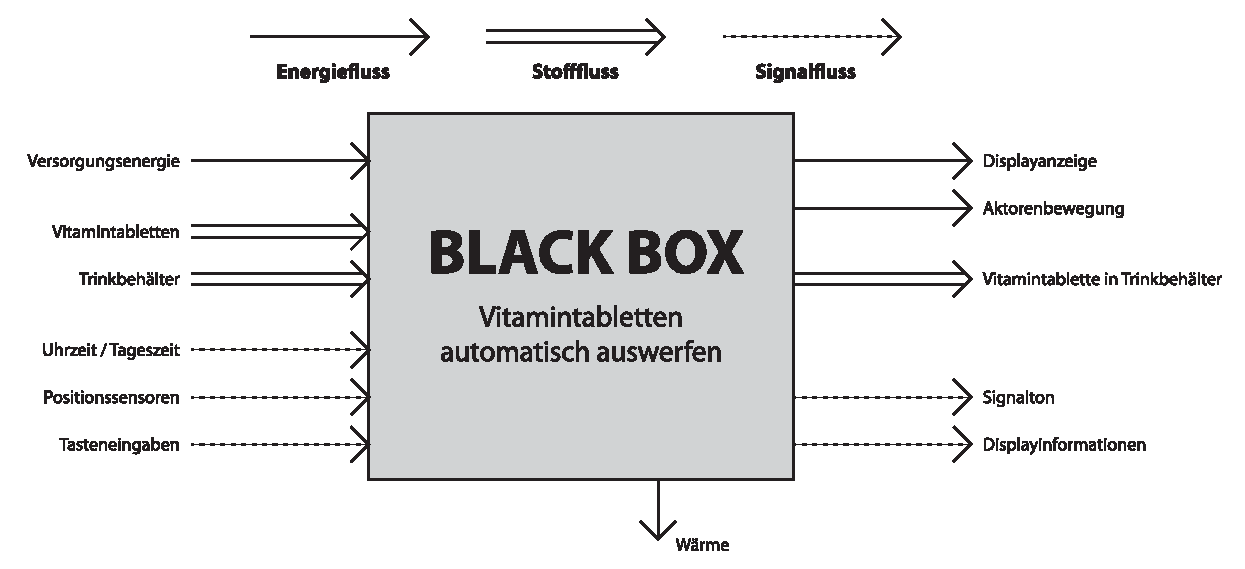
\includegraphics[width=1.0\linewidth]{../drawings/funktionsstruktur_kybernetisch}
	\caption{Allgemeine kybernetische Black-Box-Darstellun}
	\label{fig:funktionsstrukturkybernetisch}
\end{figure}

\begin{figure}[H]
	\centering
	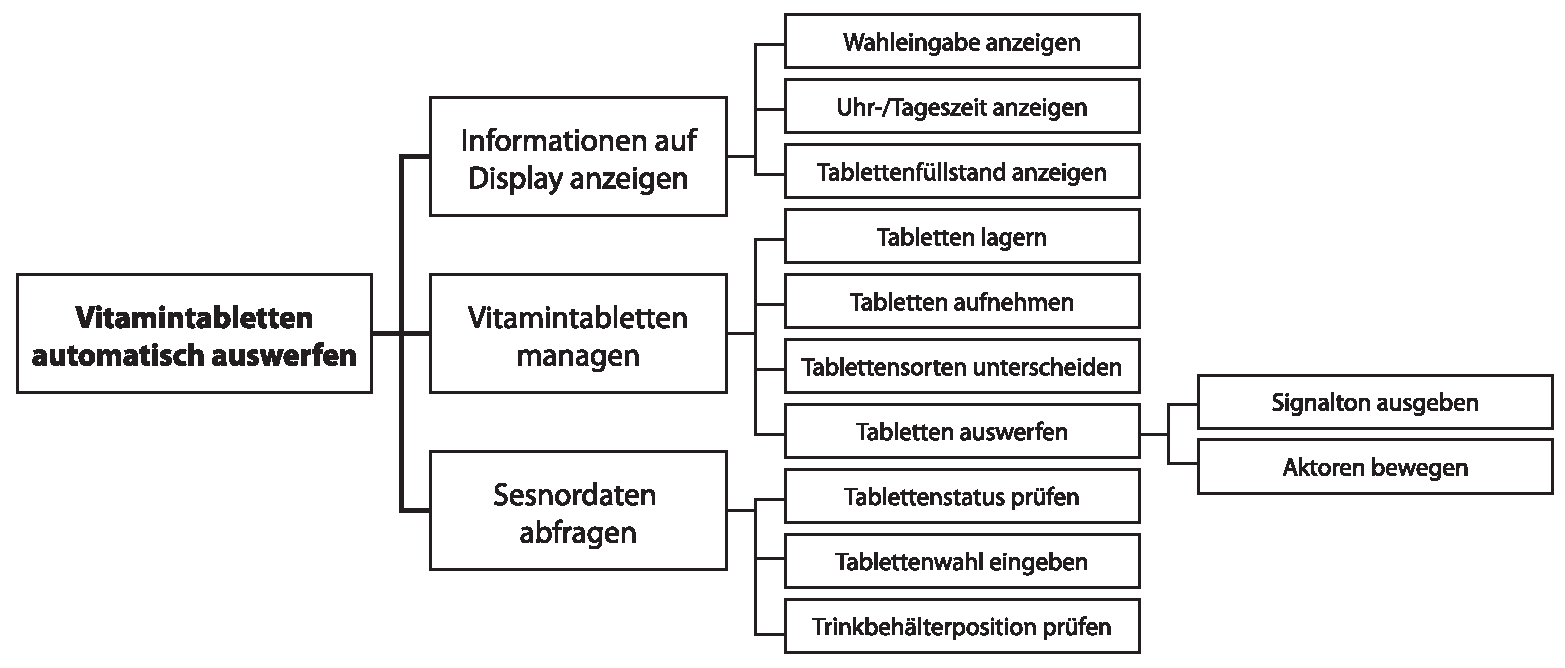
\includegraphics[width=1.0\linewidth]{chapter/Bilder/funktionsstruktur_hierarchisch}
	\caption{Hierarchische Funktionsstruktur}
	\label{fig:funktionsstrukturhierarchisch}
\end{figure}

\begin{figure}[H]
	\centering
	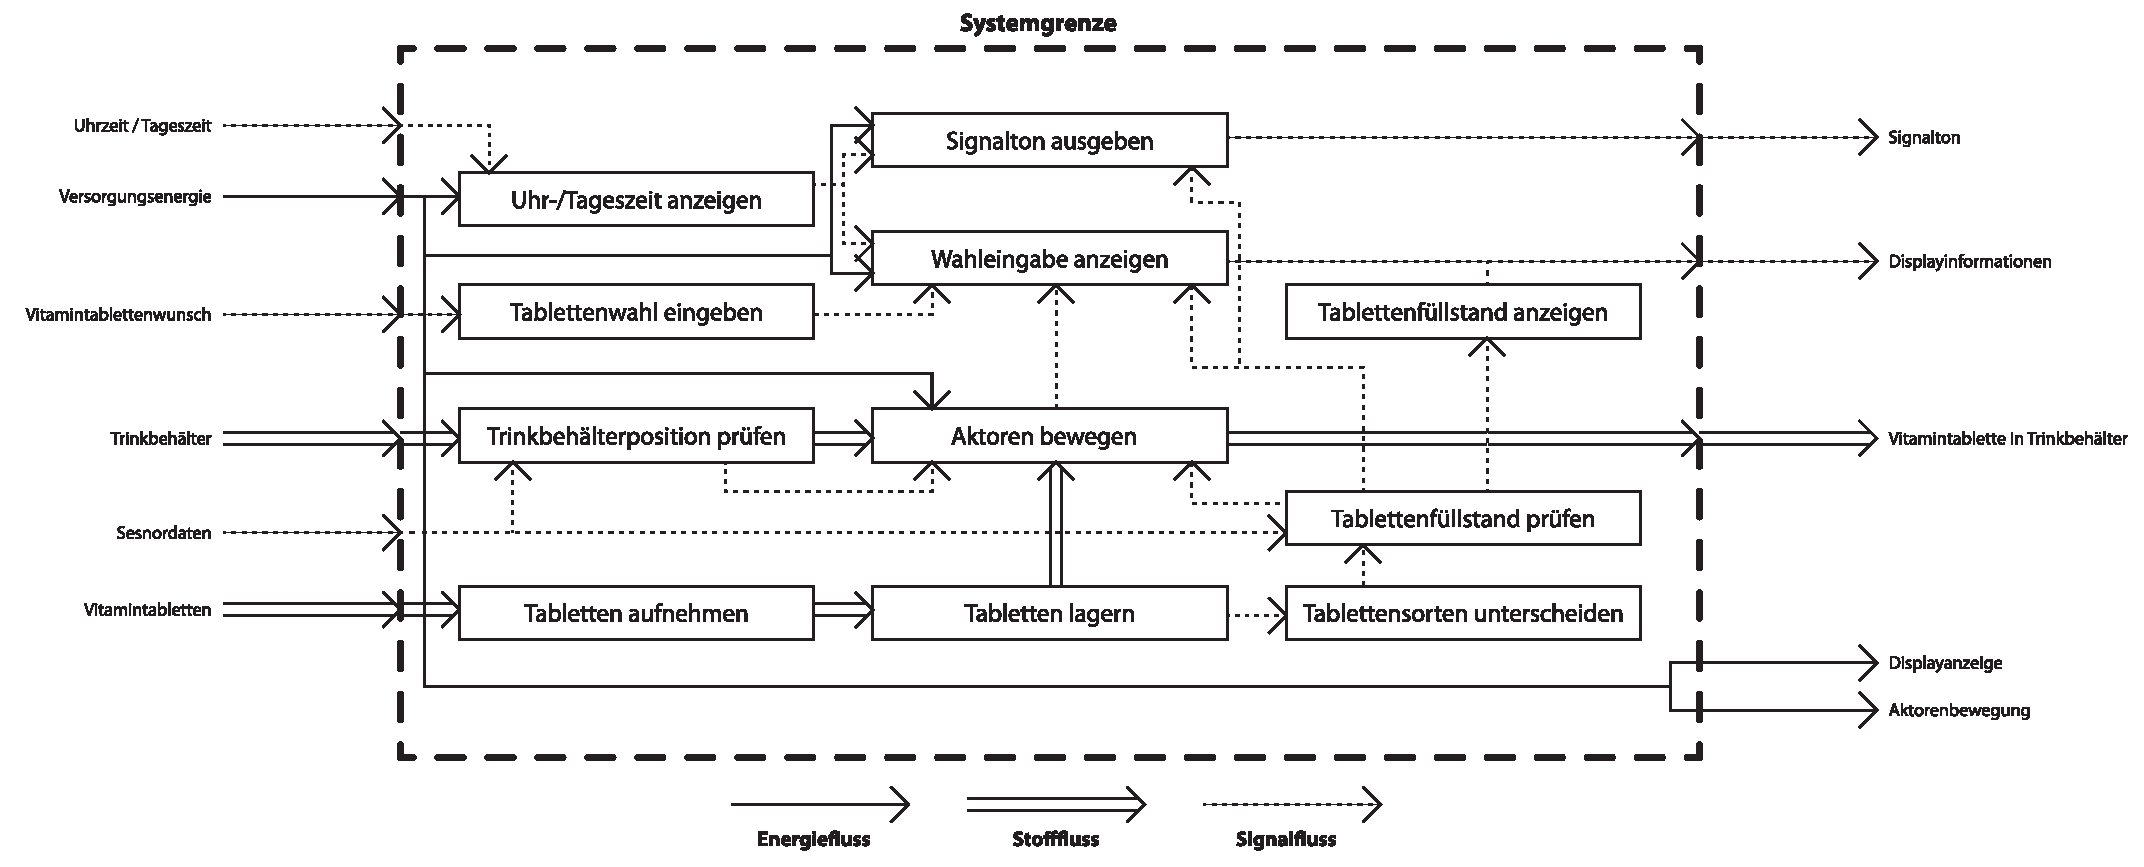
\includegraphics[angle=90, height=0.9\textheight]{chapter/Bilder/funktionsmodell}
	\caption{Funktionsmodell mit Darstellung der  wichtigsten Funktionen}
	\label{fig:funktionsmodell}
\end{figure}

\newpage
\section{Lösungsprinzipien}

\begin{figure}[H]
	\centering
	\includegraphics[width=1.0\linewidth]{chapter/Bilder/morphkasten}
	\caption{Morphologischer Kasten}
	\label{fig:morphkasten}
\end{figure}

\begin{figure}[H]
	\centering
	\includegraphics[width=1.0\linewidth]{chapter/Bilder/vertraeglichkeit}
	\caption{Verträglichkeitsmatrix}
	\label{fig:vertraglichkeit}
\end{figure}

\begin{figure}[H]
	\centering
	\includegraphics[width=1.0\linewidth]{chapter/Bilder/loesungskombinationen}
	\caption{Kennzeichnungen von 4 möglichen Gesamtlösungskombinationen}
	\label{fig:losungskombinationen}
\end{figure}

\begin{figure}[H]
	\centering
	\includegraphics[width=1.0\linewidth]{chapter/Bilder/nutzwertanalyse}
	\caption{Gesamtlösungskombinaiton Bewertung}
	\label{fig:nutzwertanalyse}
\end{figure}

\newpage
\section{Technische Prinzipskizze}

\begin{figure}[H]
	\centering
	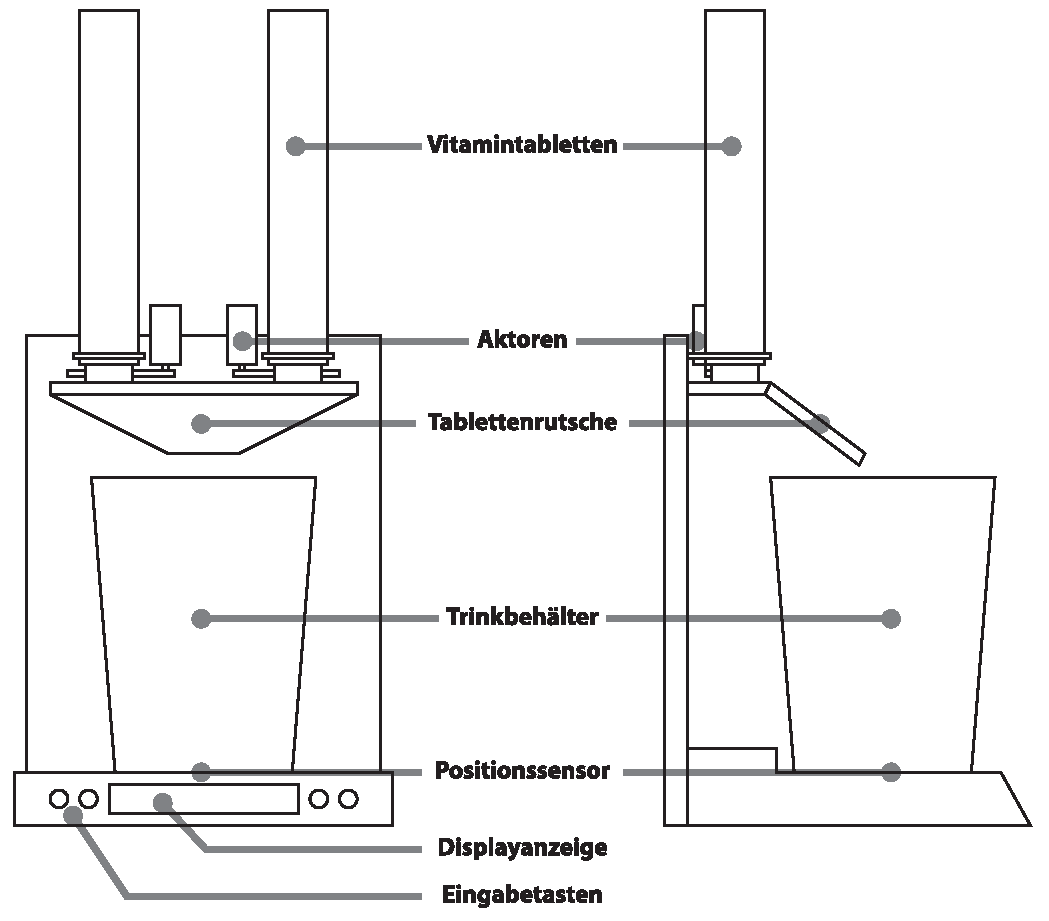
\includegraphics[width=1.0\linewidth]{chapter/Bilder/schematic_bw}
	\caption{Technische Funktionsskizze (links Vorderansicht, rechts Seitenansicht)}
	\label{fig:schematicbw}
\end{figure}

Diese technische Funktionsskizze zeigt den geplanten Aufbau unserer Apparatur. Zentral zu sehen ist der Trinkbehälter, dessen Positionierung automatisch erkannt wird. Darunter ist ein kleines Display, welche wichtige Informationen anzeigt. Über dem Trinkbehälter befindet sich das Herzstück, die Vitamintabletten mit einem Servogesteuerten automatischen Auswurfmechanismus.
